\subsection{Extreme Gradient Boosting}

\begin{frame}{Extreme Gradient Boosting}
    Intro
\end{frame}

\begin{frame}{Features}
    \begin{figure}[h]
		\centering
		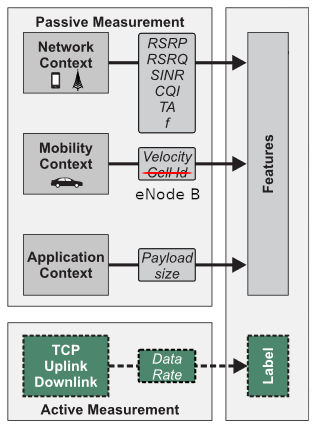
\includegraphics[height=0.75\textheight]{grafiken/features}
		\caption{Modellfeatures \cite{IEEE}.}
		\label{features}
	\end{figure}
\end{frame}

\begin{frame}{Validierung}
	\begin{figure}[h]
		\centering
		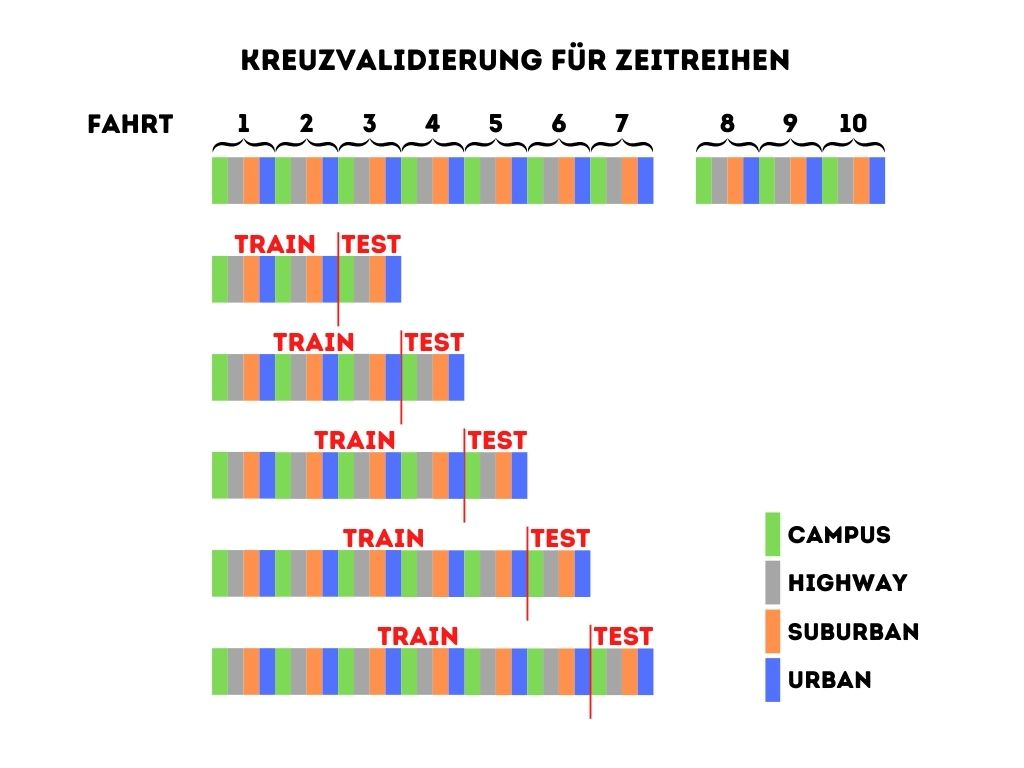
\includegraphics[scale=0.33]{kreuzvalidierung}
		\caption{Einteilungen in Trainings- und Testdatensätze bei der Kreuzvalidierung für Zeitreihen.}
		\label{kreuzvalidierung}
	\end{figure}
\end{frame}

\begin{frame}{Tuning}
    \textbf{Suchraum der Hyperparameter:}
    \begin{itemize}
        \item Anzahl der Boosting Runden $n\_rounds \in [100, 1000]$
        \item \glqq Shrinkage \grqq{} Faktor (Lernrate) $\eta \in [0.01, 1]$
        \item Strafterm f\"ur Anzahl Baumbl\"atter $\gamma \in [0, 10]$
        \item Strafterm f\"ur Vorhersagen der Baumbl\"atter $\lambda \in [0, 10]$
    \end{itemize}
    \textbf{$\Rightarrow$ Randomisierte Gittersuche}
    \begin{itemize}
        \item 20 Gitterpunkte in jeder Dimension
        \begin{itemize}
            \item[$\Rightarrow$] Insgesamt $20^4 = 160.000$ Gitterpunkte
        \end{itemize}
        \item Ausgewertet an 50 zuf\"alligen Stellen
        \item Berechnung des MAE mit Zeitreihenkreuzvalidierung f\"ur die Fahrten 1-7
    \end{itemize}
\end{frame}

\begin{frame}{Out-of-Sample Vorhersagen Upload}
    \begin{figure}[h]
        \centering
        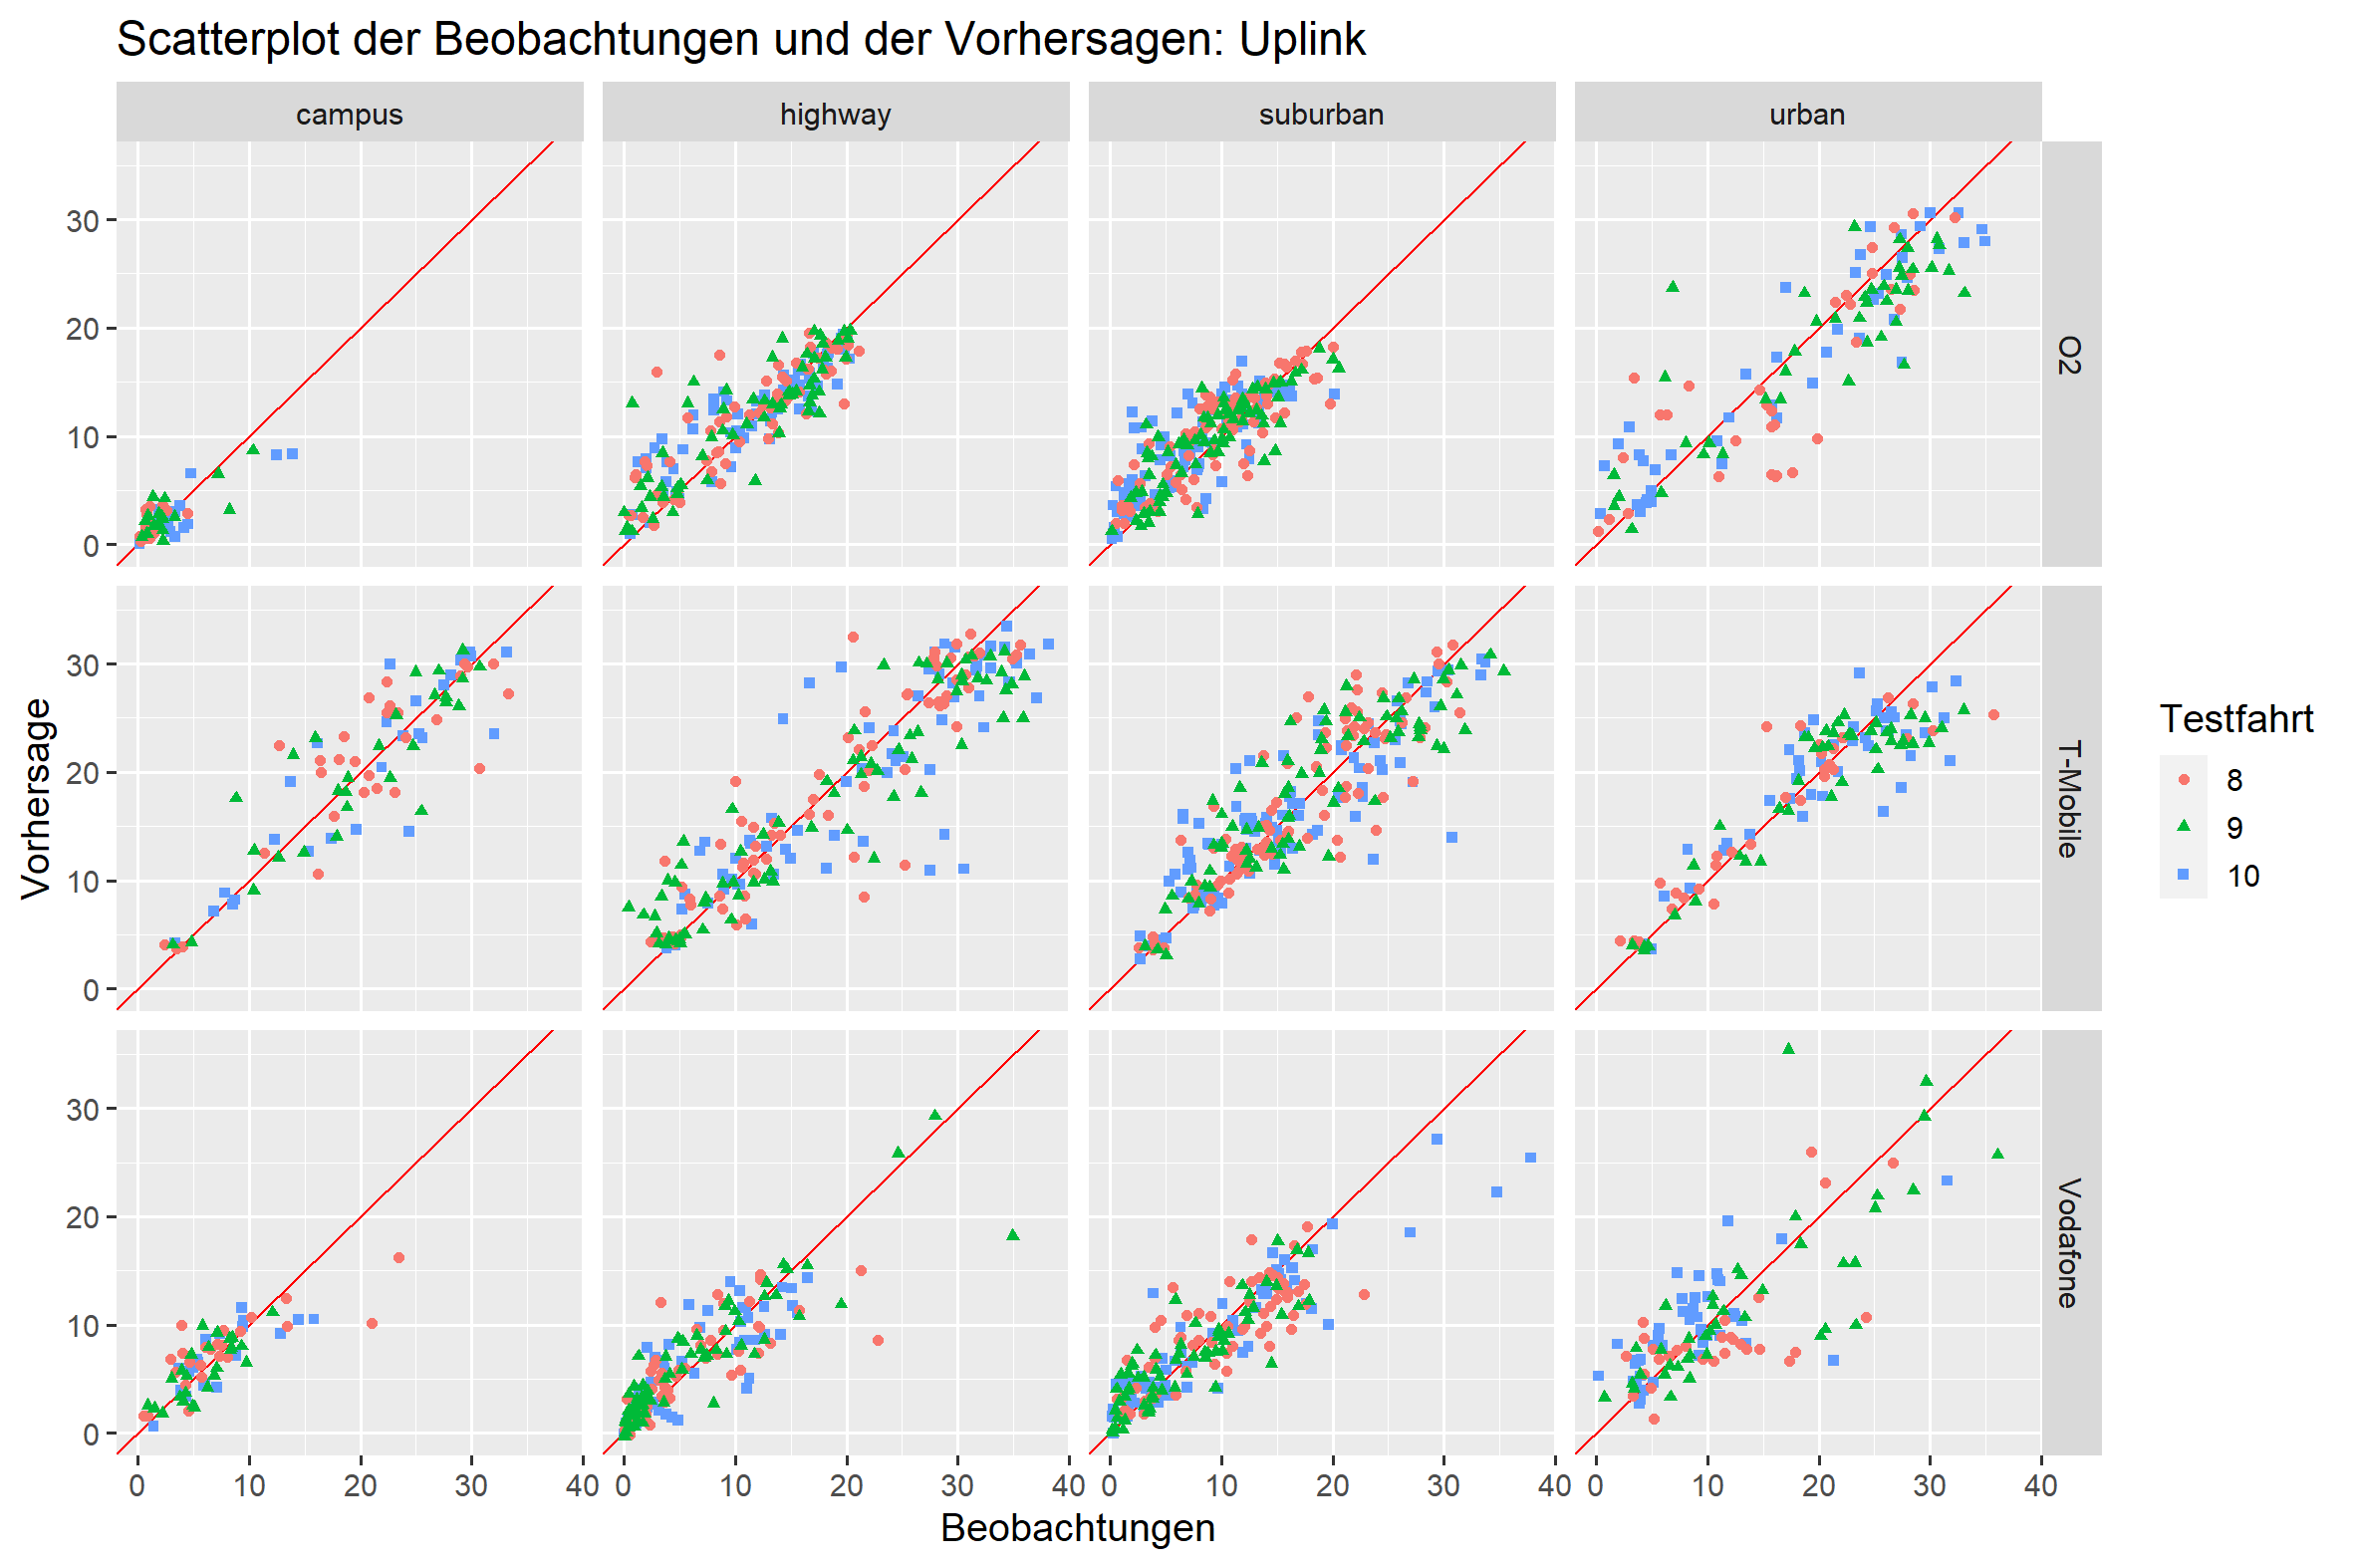
\includegraphics[scale=0.33]{plots/xgboost/uplink/scatter_colored_axes_fixed}
        \caption{XGBoost Out-of-Sample Vorhersagen der Upload-Rate}
        \label{xgboost_scatter_colored_uplink}
    \end{figure}
\end{frame}

\begin{frame}{Out-of-Sample Vorhersagen Download}
    \begin{figure}[h]
        \centering
        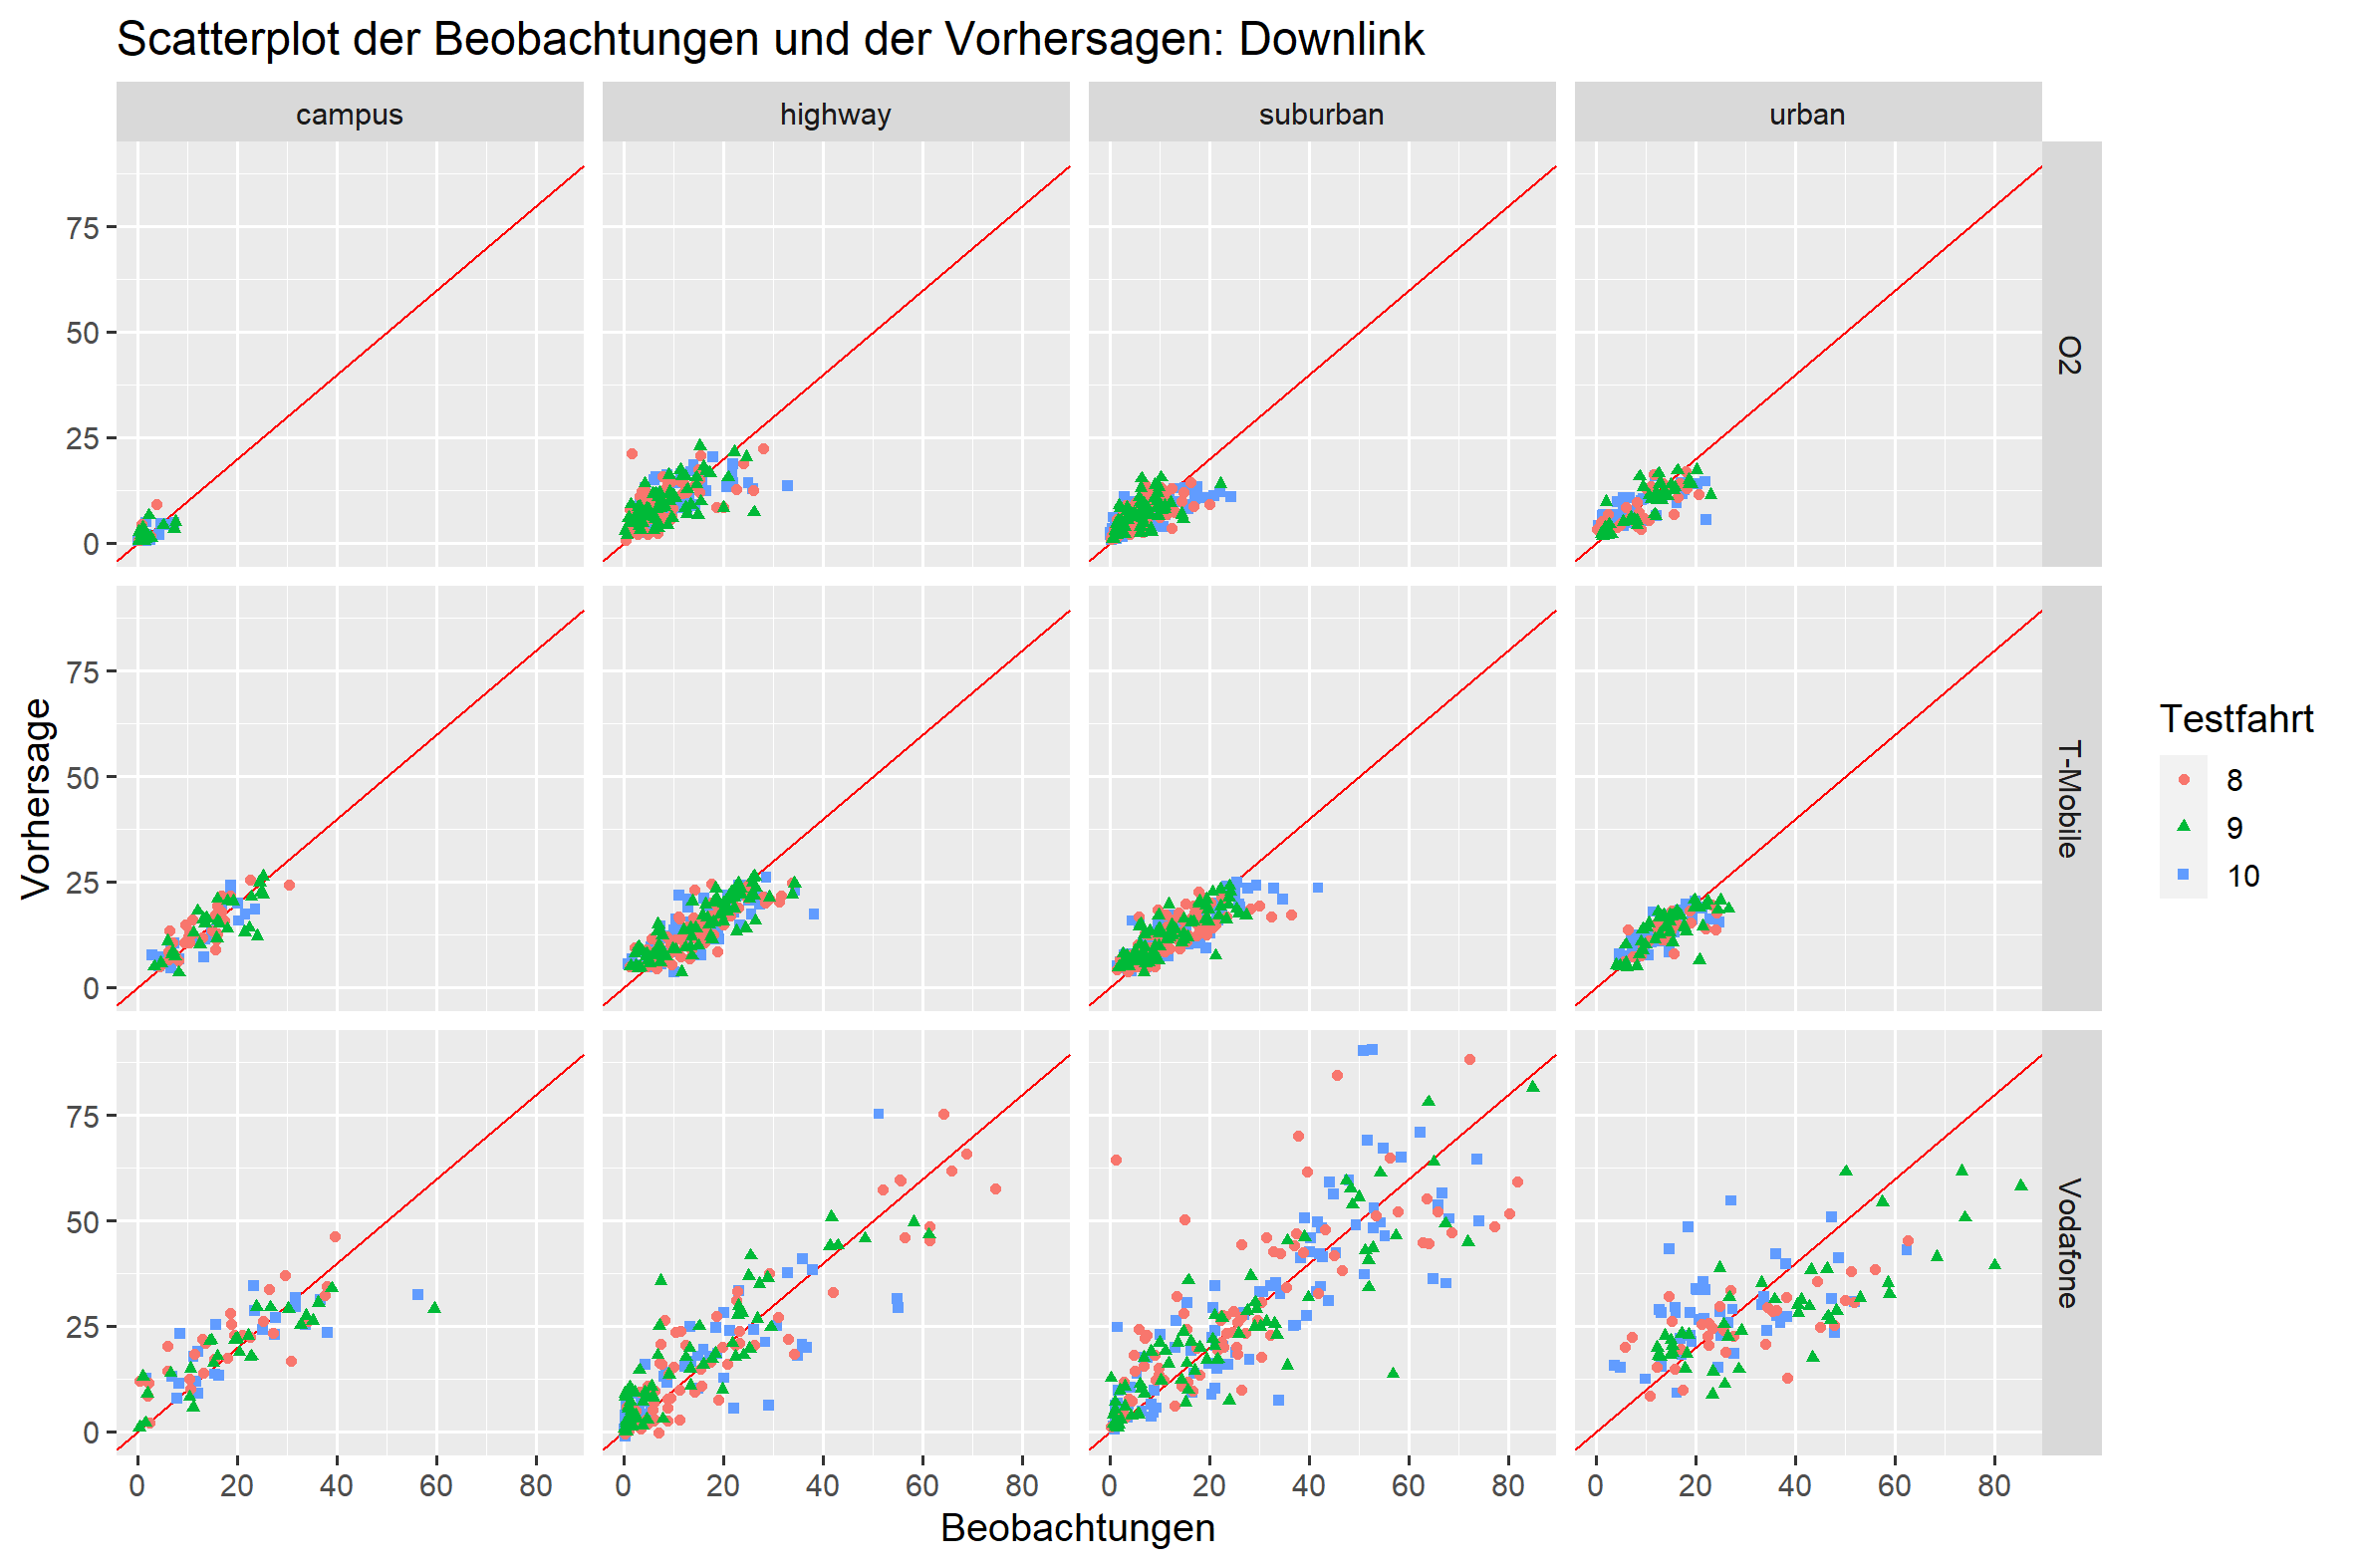
\includegraphics[scale=0.33]{plots/xgboost/downlink/scatter_colored_axes_fixed}
        \caption{XGBoost Out-of-Sample Vorhersagen der Download-Rate}
        \label{xgboost_scatter_colored_downlink}
    \end{figure}
\end{frame}